\section{Create a module}

このチュートリアルは、Go言語の基本的な機能をいくつか紹介する最初の部分です。Go を使い始めたばかりの方は、チュートリアルをぜひご覧ください。
Go を使い始めたばかりという方は、チュートリアル: 「Go を使い始める」をご覧ください。これは、go コマンド、Go モジュール、および非常に簡単な Go コードを紹介しています。

このチュートリアルでは、2つのモジュールを作成します。1つ目はライブラリで、他のライブラリやアプリケーションからインポートされることを想定しています。2つ目は、1つ目のモジュールを使用する呼び出し側のアプリケーションです。

このチュートリアルでは、言語の異なる部分を説明する7つの簡単なトピックを用意しています。

\begin{enumerate}
\item モジュールを作成する -- 他のモジュールから呼び出せる関数を含む小さなモジュールを書く。
\item 他のモジュールからあなたのコードを呼び出す -- 新しいモジュールをインポートして使用する。
\item エラーを返す、処理する -- 簡単なエラー処理を追加する。
\item ランダムな挨拶を返す -- スライス(Goの動的サイズ配列)でデータを処理する。
\item 複数人のあいさつを返す -- キーと値のペアをマップに格納する。
\item テストを追加する -- Goの組み込みユニットテスト機能を使って、コードをテストする。
\item アプリケーションをコンパイルしてインストールする -- コードをローカルにコンパイルしてインストールします。
\end{enumerate}

\subsection{前提条件}

\begin{itemize}
\item \textbf{プログラミングの経験があること。}このコードは非常にシンプルですが、関数、ループ、配列について知っておくと役に立ちます。
\item \textbf{コードを編集するためのツール。}あなたが持っているどんなテキストエディタでも大丈夫です。ほとんどのテキストエディタがGoをうまくサポートしています。VSCode(無料)、GoLand(有料)、Vim(無料)などが有名です。
\item \textbf{コマンドターミナル。}LinuxやMacではターミナルを、WindowsではPowerShellやcmdを使うとうまく動きます。
\end{itemize}

\subsection{他の人が使えるモジュールを始める}

まずはGoモジュールを作成することから始めましょう。モジュールでは、1つまたは複数の関連するパッケージを集めて、個別の有用な機能の集合を作成します。たとえば、財務分析を行う関数を持つパッケージでモジュールを作成し、財務アプリケーションを書いている他の人があなたの仕事を利用できるようにすることができます。モジュールの開発について詳しくは、「モジュールの開発と公開」を参照してください。

Go のコードはパッケージにまとめられ、パッケージはモジュールにまとめられます。モジュールは、コードの実行に必要な依存関係(Go バージョンや必要な他のモジュールのセットなど)を指定します。

モジュールの機能を追加または改善したら、モジュールの新バージョンを公開します。モジュールの関数を呼び出すコードを書いている開発者は、モジュールの更新されたパッケージをインポートして、実運用に移す前に新しいバージョンでテストすることができます。


\begin{enumerate}
\item コマンドプロンプトを開き、ホームディレクトリに\texttt{cd}してください。

LinuxまたはMacの場合。
\begin{lstlisting}[numbers=none]
cd
\end{lstlisting}
Windowsの場合。
\begin{lstlisting}[numbers=none]
cd %HOMEPATH%
\end{lstlisting}

\item Goモジュールのソースコードを格納する\texttt{greetings}ディレクトリを作成します。

例えば、ホームディレクトリから以下のコマンドを使用します。
\begin{lstlisting}[numbers=none]
mkdir greetings
cd greetings
\end{lstlisting}

\item \texttt{go mod init}コマンドでモジュールを起動します。

\texttt{go mod init}コマンドを実行し、モジュールのパスを指定します -- ここでは\texttt{example.com/greetings}を使用します。モジュールを公開する場合は、Goツールでモジュールをダウンロードできるパスである必要があります。これはあなたのコードのリポジトリになります。

モジュールパスによるモジュールの命名の詳細については、依存関係の管理 を参照してください。

\begin{lstlisting}[numbers=none]
$ go mod init example.com/greetings
go: creating new go.mod: module example.com/greetings
\end{lstlisting}

\texttt{go mod init}コマンドは、あなたのコードの依存関係を追跡するために\texttt{go.mod}ファイルを作成します。今のところ、このファイルにはモジュールの名前とコードがサポートするGoのバージョンだけが含まれています。しかし、依存関係を追加すると、\texttt{go.mod} ファイルはあなたのコードが依存するバージョンをリストアップします。これにより、ビルドの再現性が保たれ、使用するモジュールのバージョンを直接制御することができます。

\item テキストエディタで、コードを記述するためのファイルを作成し、greetings.goとします。

\item 以下のコードをgreetings.goファイルに貼り付けて保存してください。

\begin{lstlisting}[numbers=none]
package greetings

import "fmt"

// Hello returns a greeting for the named person.
func Hello(name string) string {
    // Return a greeting that embeds the name in a message.
    message := fmt.Sprintf("Hi, %v. Welcome!", name)
    return message
}
\end{lstlisting}

これは、あなたのモジュールの最初のコードです。これは、あいさつを要求した呼び出し側に対して、あいさつを返します。次のステップで、この関数を呼び出すコードを書きます。

このコードでは、あなたは
\begin{itemize}
\item greeting パッケージを宣言し、関連する関数を収集する。
\item 挨拶を返すHello関数を実装する。

この関数は、nameパラメータを受け取り、その型は\texttt{string}である。また、この関数は文字列を返します。Go では、名前が大文字で始まる関数は、同じパッケージに含まれない関数から呼び出すことができます。これはGoではエクスポートされた名前として知られています。エクスポートされた名前の詳細については、Go ツアーの「エクスポートされた名前」を参照してください。

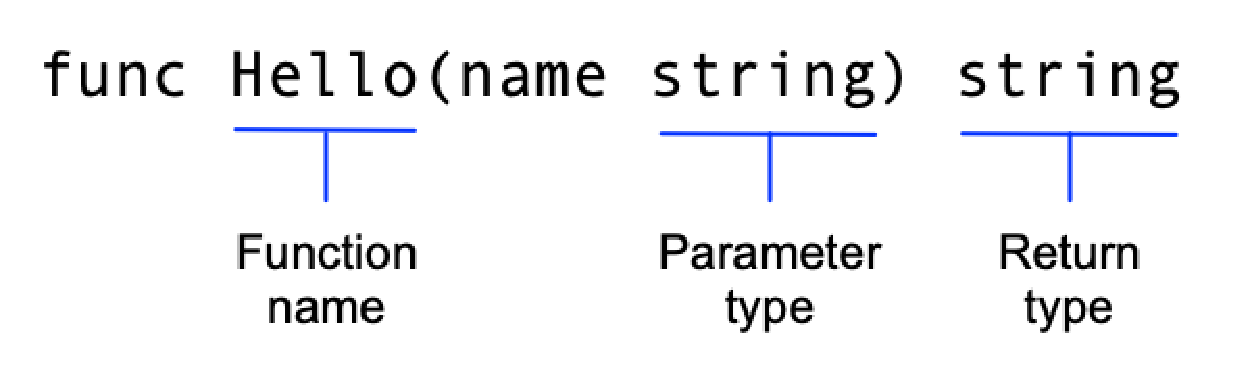
\includegraphics[width=8cm]{function-syntax.eps}

\item 挨拶を格納するメッセージ変数を宣言します。

Goでは、\texttt{:=}演算子は変数の宣言と初期化を一行で行うためのショートカットです(Goは右側の値を使って変数の型を決定します)。遠回りになりますが、次のように書いたかもしれません。

\begin{lstlisting}[numbers=none]
var message string
message = fmt.Sprintf("Hi, %v. Welcome!", name)
\end{lstlisting}

\item \texttt{fmt}パッケージの\texttt{Sprintf}関数を使用して、挨拶文を作成します。最初の引数はフォーマット文字列で、\texttt{Sprintf}は\texttt{name}パラメータの値を\texttt{\%v}フォーマット動詞に代入します。nameパラメータの値を挿入すると、挨拶文が完成する。

\item 書式設定された挨拶文を呼び出し元に返す。

\end{itemize}
\end{enumerate}


次のステップでは、別のモジュールからこの関数を呼び出すことになります。